%!TEX root = ../../super_main.tex

\section{Human Activity Recognition}
\label{sec:human_activity_recognition}

Since we want to provide data for reality mining, we must consider how we want to approach human activity recognition. There are at least two overall different approaches to this namely participatory and opportunistic sensing \parencite{opp_or_par} \parencite{har_wearables}. Participatory sensing requires that a participant actively participates in the data collection by own initiative as illustrated in \figref{fig:participatory_sensing}, directly entering data, or by otherwise reacting to requests for input. Opportunistic sensing requires less to none involvement from the participant, but it does require more passive monitoring of the context of the participant even when the system is not actively gathering data in order to sense if the participant's context matches triggering conditions as seen in \figref{fig:opportunistic_sensing}. 

\begin{figure}[!htbp]
\begin{subfigure}[!t]{.45\textwidth}
  \centering
  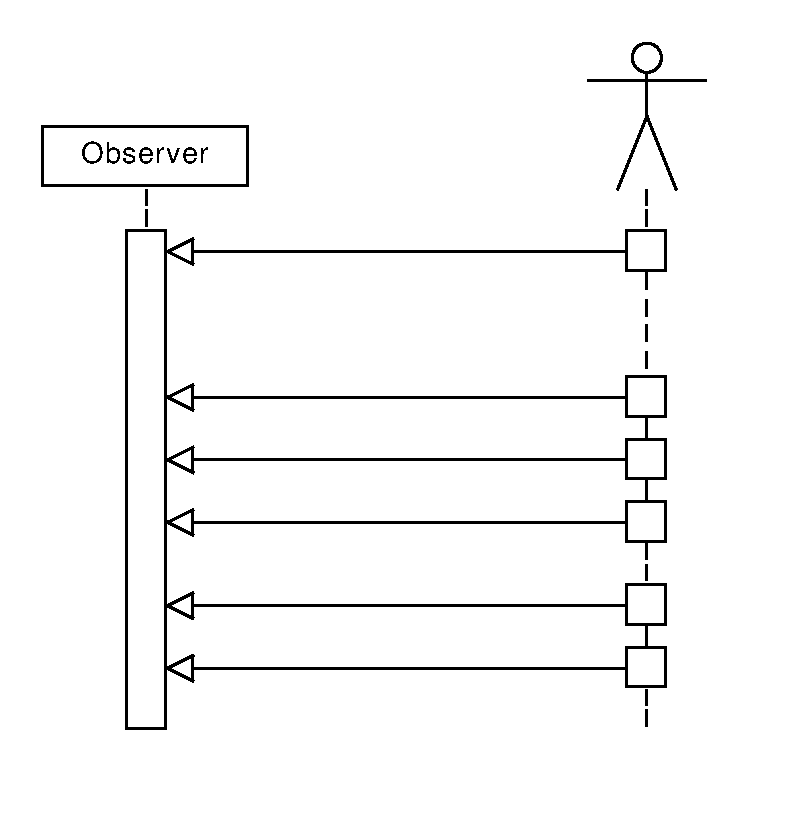
\includegraphics[width=\linewidth]{problem_analysis/opportunistic_sensing}
  \caption{Opportunistic sensing.}
  \label{fig:opportunistic_sensing}
\end{subfigure}
~
\begin{subfigure}[!t]{.45\textwidth}
  \centering
  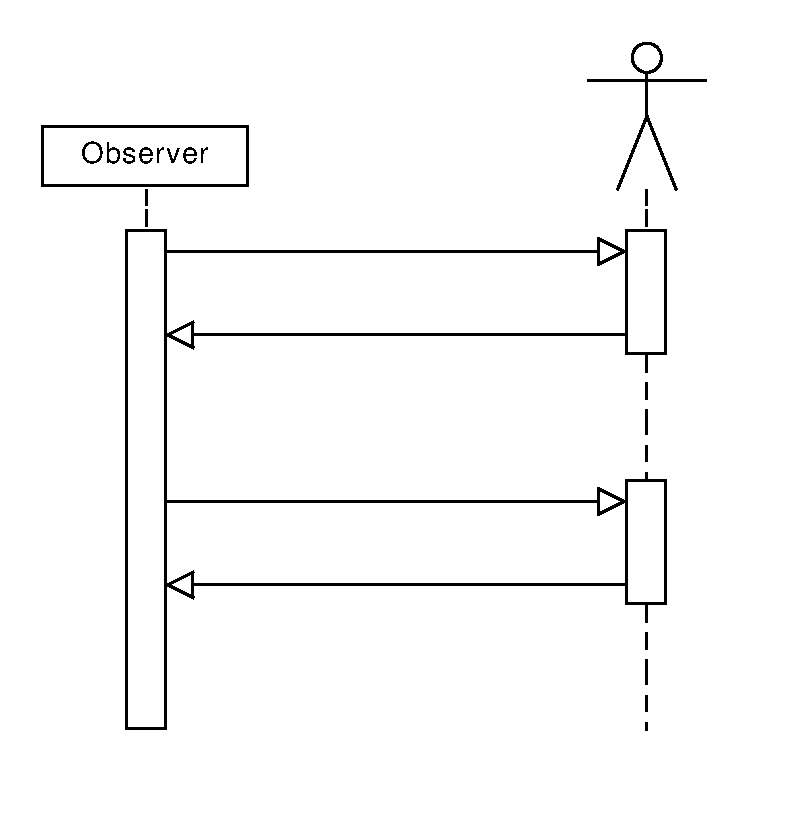
\includegraphics[width=\linewidth]{problem_analysis/participatory_sensing}
  \caption{Participatory sensing.}
  \label{fig:participatory_sensing}
\end{subfigure}
\caption{Two ways of sensing the human activity.}
\label{fig:sensing_types}
\end{figure}
\FloatBarrier

A platform that performs opportunistic sensing for reality mining would have to actively monitor, or somehow be aware of, when participants are physically located near an area of interest. A configuration of a campaign, as defined by AndWellness, see \secref{sub:andwellness}, is somewhat analogous with the  term application query of \parencite{opp_or_par}. Such a blueprint for the data collection part of reality mining, seems to be a general concept across different solutions. A data collection blueprint could for instance require that data should be gathered when the participant is drinking coffee, i.e. they are near a coffee shop. This constant monitoring of the participants context, in order to enable triggers, might though present its own privacy intrusion problems. This monitoring could however be performed locally on the mobile devices of the participants, and their privacy could thus be somewhat preserved, because this additional monitoring data will not be shared with others. 
\\\\
The two approaches can be combined where opportunistic sensing could capture the context, at opportune times, in the shape of values read from sensors. Participatory sensing could be used to include participants by allowing them to provide labels for the same data set. The participatory sensing could be triggered, when certain conditions are met during the opportunistic sensing, which could be defined by the customers. This would allow customers to configure a campaign and specify to which degree they want participant involvement, i.e. participatory sensing, and when and how they want it, i.e. opportunistic sensing.
\\\\
The amount of different labels one could infer directly from the sensor data is somewhat limited and would not allow many possible labels which capture human behavior or state. One could attempt to setup artificial rules and infer labels for the data based on these rules; these rules would however likely be based on assumptions about the data, unless some other ground truth is known. It would be difficult to infer possibly interesting types of human behavior, physical state, or mental state, such as stress levels or happiness, without human involvement to define labels. One might however, with a given algorithm or machine intelligence model, be able to recognize patterns in the data to infer labels, this could for instance be if the person is dancing or not, e.g. by detecting rhythmic movement.    
\newpage
One way to involve participants could be through questionnaires with one or more questions. The answers could then determine the labels of the data. The validity of this participant generated data would depend on the truthfulness and perception of the participants, which could be a source of error. The validity of the data could however be evaluated and filtered by customers outside the data collection system. Data from external sensors or other certain combinations of values from the collected set of features, might be helpful in determining the validity of answers provided by participants. An example could be a data set with accelerometer readings that clearly show that the participant was not moving, but he answers in the questionnaire that he was running. 
\\\\
We will need to support some kind of participant involvement in order to be able to gather labels for the participants context. The success of the system thus partially depends on how willing participants are to participate, first by actually installing the data gathering application, and secondly how actively participants are willing to contribute and provide labels to pair with the captured contexts. It is thus up to the customers to design campaigns the participants are willing to participate in. The success of the system therefore depends on a combination of the persuasiveness of the customers, and the ability of the system to let customers specify campaigns that participants are willing to contribute to.
